\documentclass[a4paper, 11pt]{article}
\usepackage[utf8]{inputenc}
\usepackage{amsmath}
\usepackage{array}
\usepackage{listings}
\usepackage{color}
\usepackage{booktabs}
\usepackage{subcaption}
\usepackage{caption}
\usepackage{varioref}
\usepackage[section]{placeins}
\usepackage{comment} % enables the use of multi-line comments (\ifx \fi) 
\usepackage{graphicx}
\usepackage{lipsum} %This package just generates Lorem Ipsum filler text. 
\usepackage{fullpage} % changes the margin
\usepackage{cleveref}
\definecolor{dkgreen}{rgb}{0,0.6,0}
\definecolor{gray}{rgb}{0.5,0.5,0.5}
\definecolor{mauve}{rgb}{0.58,0,0.82}

\DeclareMathOperator*{\argmax}{argmax} % thin space, limits underneath in displays

\newenvironment{conditions}
{\par\vspace{\abovedisplayskip}\noindent\begin{tabular}{>{$}l<{$} @{${}={}$} l}}
	{\end{tabular}\par\vspace{\belowdisplayskip}}

\renewcommand{\lstlistingname}{Algorithm}% Listing -> Algorithm
\renewcommand{\lstlistlistingname}{List of \lstlistingname s}% List of Listings -> List of Algorithms
\crefname{listing}{algorithm}{algorithms}  
\Crefname{listing}{Algorithm}{Algorithms}

\lstset{frame=tb,
	language=Python,
	aboveskip=3mm,
	belowskip=3mm,
	showstringspaces=false,
	columns=flexible,
	basicstyle={\small\ttfamily},
	numbers=left,
	numberstyle=\tiny\color{gray},
	keywordstyle=\color{blue},
	commentstyle=\color{dkgreen},
	stringstyle=\color{mauve},
	breaklines=true,
	breakatwhitespace=true,
	tabsize=3,
	inputencoding=latin1
}

\captionsetup[figure]{skip=0pt}

\begin{document}
	%Header-Make sure you update this information!!!!
	\noindent
	\large\textbf{Homework 3 Report} \hfill \textbf{Piero Macaluso s252894} \\
	\normalsize Machine Learning and Artificial Intelligence 2018/2019 \hfill Prof. Barbara Caputo  \\
	\normalsize Politecnico di Torino \hfill Due Date: 19/01/2019 
	
	 
	\section*{Deep Learning Setup}
	For this homework, I set up the environment on my personal laptop: the durations shown in the report refer to the following specifications. The dataset used in this homework is \textbf{CIFAR-100}.
	\subsection*{Hardware}
	\begin{itemize}
		\item \textbf{Laptop Model} Dell Inspiron 7559
		\item \textbf{CPU} Intel® Core™ i7-6700HQ CPU @ 2.60GHz x 8 
		\item \textbf{Video Card} NVIDIA GeForce GTX 960M
		\item \textbf{RAM} 16GB
	\end{itemize}
	
	\subsection*{Software}
	\begin{itemize}
		\item \textbf{OS} Ubuntu 18.04.1 LTS
		\item \textbf{PyTorch} v. 1.0.0
		\item \textbf{TorchVision} v. 0.2.1
	\end{itemize}
	
	
	\section{Old Neural Networks} \label{oldcnn}
	
	\lstinputlisting[aboveskip=0pt,linerange={119-131},firstnumber=119,label={lst:oldcnn},caption={Old Neural Network class (\texttt{NN1.py})}]{../source_code/NN1.py}
	
	In the first part of this homework I trained a traditional neural network with 2 hidden FC (Fully connected) layers and a last FC for classification. The parameters were: \textbf{256 batch size}, \textbf{20 epochs}, \textbf{32x32 resolution}, \textbf{$\boldsymbol{0.0001}$ Adam Solver learning rate}. The class of this network is in \vref{lst:oldcnn}.
	
		\begin{figure}[ht!]
			\centering
			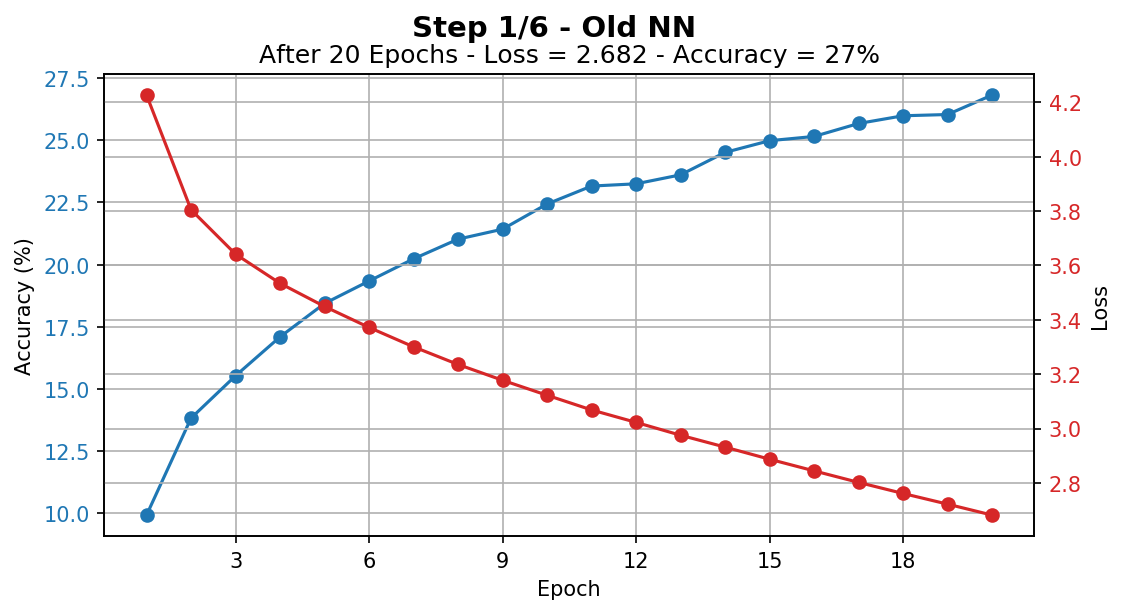
\includegraphics[width=0.65\paperwidth]{img/fig01.png}
			\caption{Old NN (loss/accuracy graph)}
			\label{fig:oldcnn}
		\end{figure}
	
	The training lasted about 5 minutes and it provided an accuracy of $\boldsymbol{27\%}$ and a loss of $\boldsymbol{2.682}$ (see \vref{fig:oldcnn}). These results are not satisfying: the accuracy is too low and the loss is high. However, I expected these results because of the NN (Neural Network) provided is implemented using only FC (Fully Connected) layers.
	
	An FC Layer links each pixel to all neurons, so it produces a large number of metric that the network has to learn. This NN can end up with \textbf{overfitting}, because the network would learn too much, without acquiring the ability to generalize on the test set. Perhaps this is the reason that led to this results.
	
	\section{Simple CNN} \label{sect2}
	
	
	In the second part of this homework I trained a CNN (Convolutional Neural Network) architecture. The parameters were: \textbf{256 batch size}, \textbf{20 epochs}, \textbf{32x32 resolution}, \textbf{$\boldsymbol{0.0001}$ Adam Solver learning rate}. The class of this network is in \vref{lst:simplecnn}.
	\lstinputlisting[aboveskip=0pt,linerange={135-154},firstnumber=135,label={lst:simplecnn},caption={Simple Convolutional Neural Network class (\texttt{CNN2.py})}]{../source_code/CNN2.py}
	\newpage
	\begin{figure}[ht!]
		\centering
		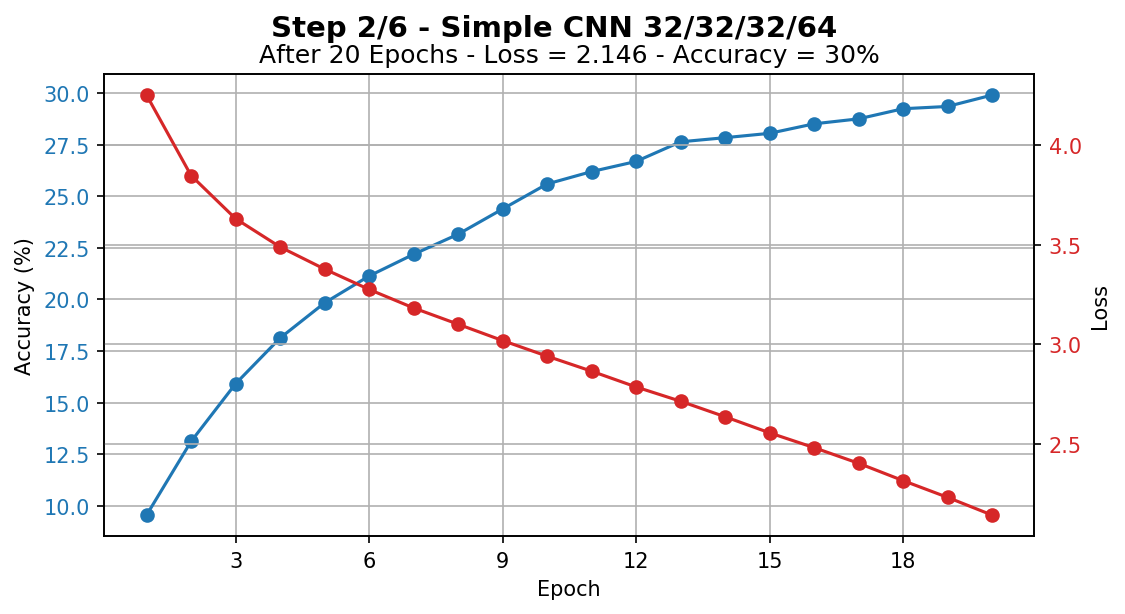
\includegraphics[width=0.65\paperwidth]{img/fig02.png}
		\caption{Simple CNN (loss/accuracy graph)}
		\label{fig:simplecnn}
	\end{figure}

	The training lasted about 2 minutes and I obtained an accuracy of $\boldsymbol{30\%}$ and a loss of $\boldsymbol{2.146}$ as wee can see in \vref{fig:simplecnn}.
	This is better than the previous NN, but not enough: the loss is still too high. This may be due, once again, to overfitting, because we are using a CNN without any type of regularization or improving techniques which could led to better results as we will see in next sections.
	
	
	\section{CNN and convolutional filters}
	
	In the third part of this homework I trained a CNN architecture using different numbers of convolutional filters. The parameters were: \textbf{256 batch size}, \textbf{20 epochs}, \textbf{32x32 resolution}, \textbf{$\boldsymbol{0.0001}$ Adam Solver learning rate}. The classes of these networks are in \vref{lst:cnn3a,lst:cnn3b,lst:cnn3c} .
	\lstinputlisting[aboveskip=0pt,linerange={135-154},firstnumber=135,label={lst:cnn3a},caption={Convolutional Neural Network 128/128/128/256 class (\texttt{CNN3a.py})}]{../source_code/CNN3a.py}
	\lstinputlisting[linerange={135-154},firstnumber=135,label={lst:cnn3b},caption={Convolutional Neural Network 256/256/256/512 class (\texttt{CNN3b.py})}]{../source_code/CNN3b.py}
	\lstinputlisting[linerange={135-154},firstnumber=135,label={lst:cnn3c},caption={Convolutional Neural Network 512/512/512/1024 class (\texttt{CNN3c.py})}]{../source_code/CNN3c.py}
	\begin{figure}[ht!]
		\centering
		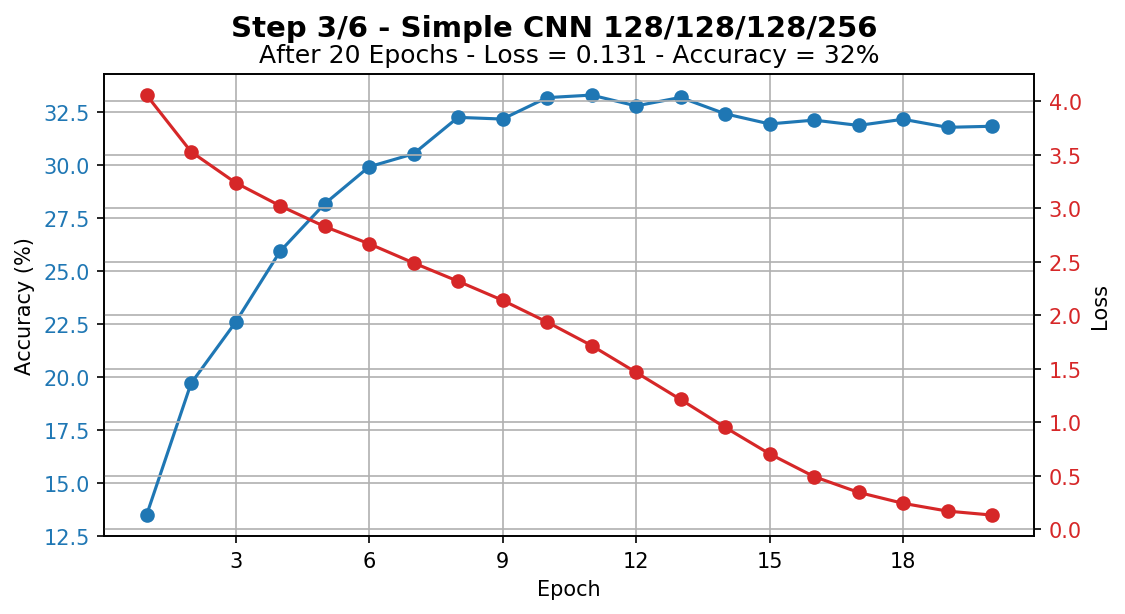
\includegraphics[width=0.6\paperwidth]{img/fig03a.png}
		\caption{CNN 128/128/128/256 (loss/accuracy graph)}
		\label{fig:03a}
	\end{figure}
	\begin{figure}[ht!]
		\centering
		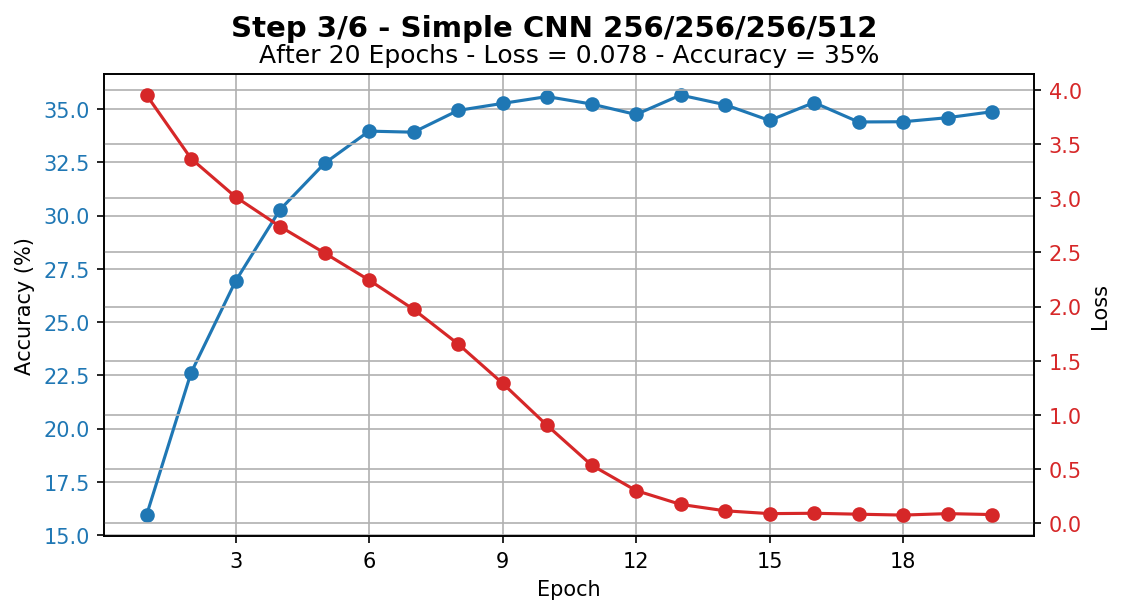
\includegraphics[width=0.6\paperwidth]{img/fig03b.png}
		\caption{CNN 256/256/256/512 (loss/accuracy graph)}
		\label{fig:03b}
	\end{figure}
	\begin{figure}[ht!]
		\centering
		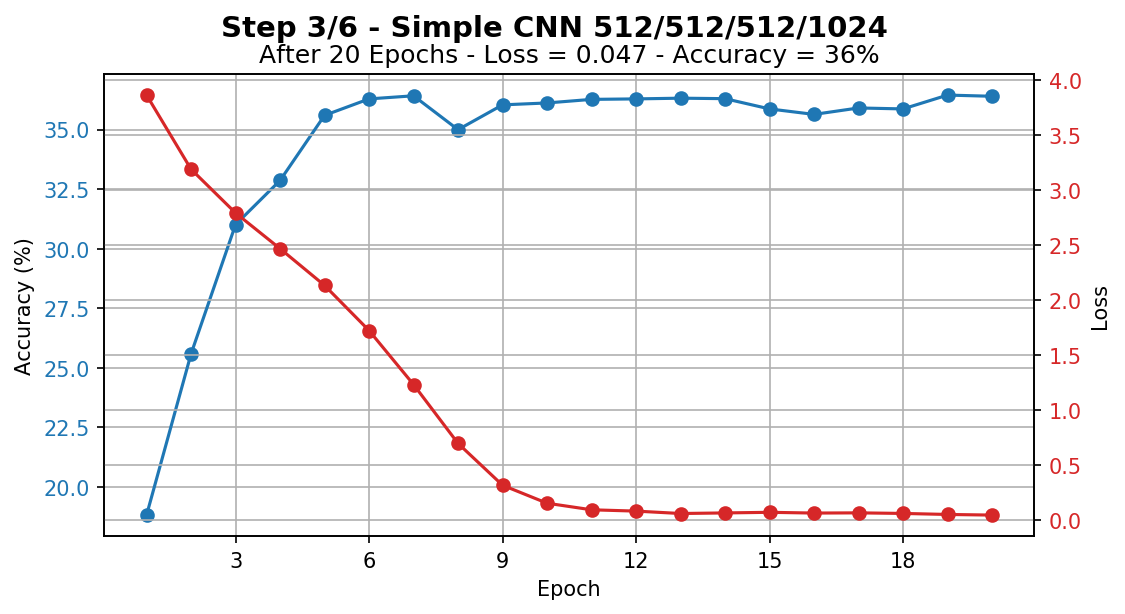
\includegraphics[width=0.6\paperwidth]{img/fig03c.png}
		\caption{CNN 512/512/512/1024 (loss/accuracy graph)}
		\label{fig:03c}
	\end{figure}
	
	The training lasted about 9 minutes for the first CNN ($\boldsymbol{32\%}$ accuracy, $\boldsymbol{0.131}$ loss)  , 25 minutes for the second one ($\boldsymbol{35\%}$ accuracy, $\boldsymbol{0.078}$ loss) and 1 hour and 15 minutes for the last one ($\boldsymbol{36\%}$ accuracy, $\boldsymbol{0.047}$ loss), as shown in \vref{fig:03a,fig:03b,fig:03c}.
	These data are better than the previous CNN ones, not only in terms of accuracy, but especially as far as concerns the loss. Accuracies are not so high, while in all three cases the loss is very close to $0$. The parameters that the network has to learn increase with the number of filters. It is clear that both curves reach an asymptote.  
	This may be due, once again, to overfitting or co-adaptation, because, as in the previous section,  we are using a CNN without any type of regularization or improving techniques, which could led to better results, as we will see in next sections.
		
	\FloatBarrier
	
	\section{Regularization and Improving techniques}
		
	\lstinputlisting[linerange={135-158},firstnumber=135,label={lst:cnn4a},caption={Convolutional Neural Network with BN (Batch Normalization) (\texttt{CNN4a.py})}]{../source_code/CNN4a.py}
	
	\lstinputlisting[linerange={135-158},firstnumber=135,label={lst:cnn4b},caption={Convolutional Neural Network with BN and FC1 wider (\texttt{CNN4b.py})}]{../source_code/CNN4b.py}
	\lstinputlisting[linerange={135-159},firstnumber=135,label={lst:cnn4c},caption={Convolutional Neural Network with BN and Dropout $0.5$ on FC1 (\texttt{CNN4c.py})}]{../source_code/CNN4c.py}
	
	In the fourth part of this homework I trained a CNN architecture using different types of regularization and improving techniques starting from the network with $128$/$128$/$128$/$256$ filters. The parameters were: \textbf{256 batch size}, \textbf{20 epochs}, \textbf{32x32 resolution}, \textbf{$\boldsymbol{0.0001}$ Adam Solver learning rate}. The classes of these networks are in \vref{lst:cnn4a,lst:cnn4b,lst:cnn4c} .
	\begin{figure}[ht!]
		\centering
		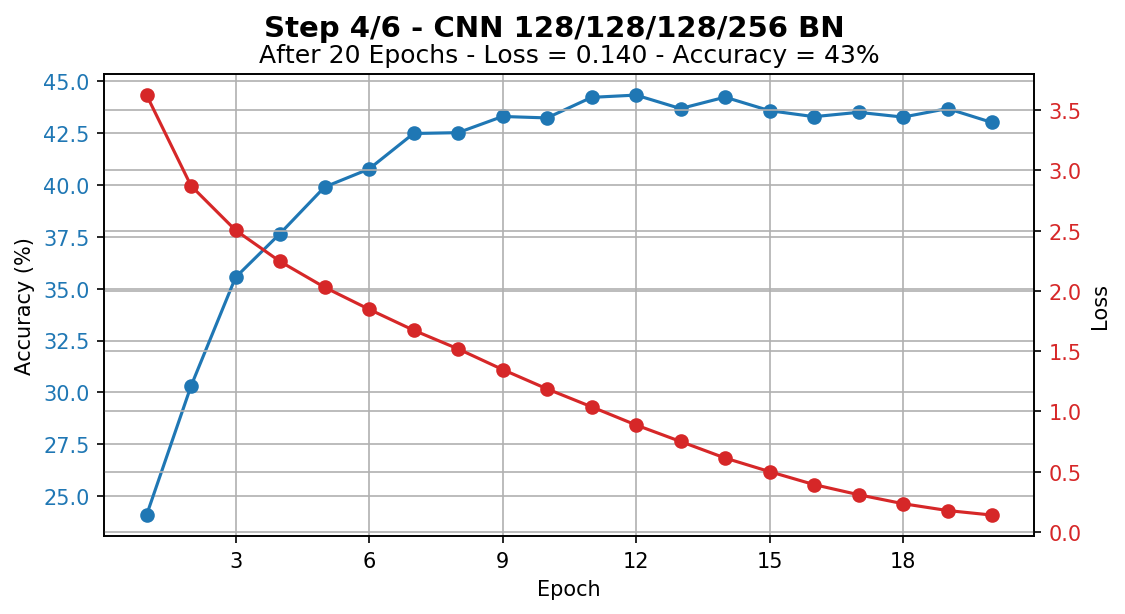
\includegraphics[width=0.62\paperwidth]{img/fig04a.png}
		\caption{CNN with Batch Normalization (loss/accuracy graph)}
		\label{fig:04a}
	\end{figure}
	\begin{figure}[ht!]
		\centering
		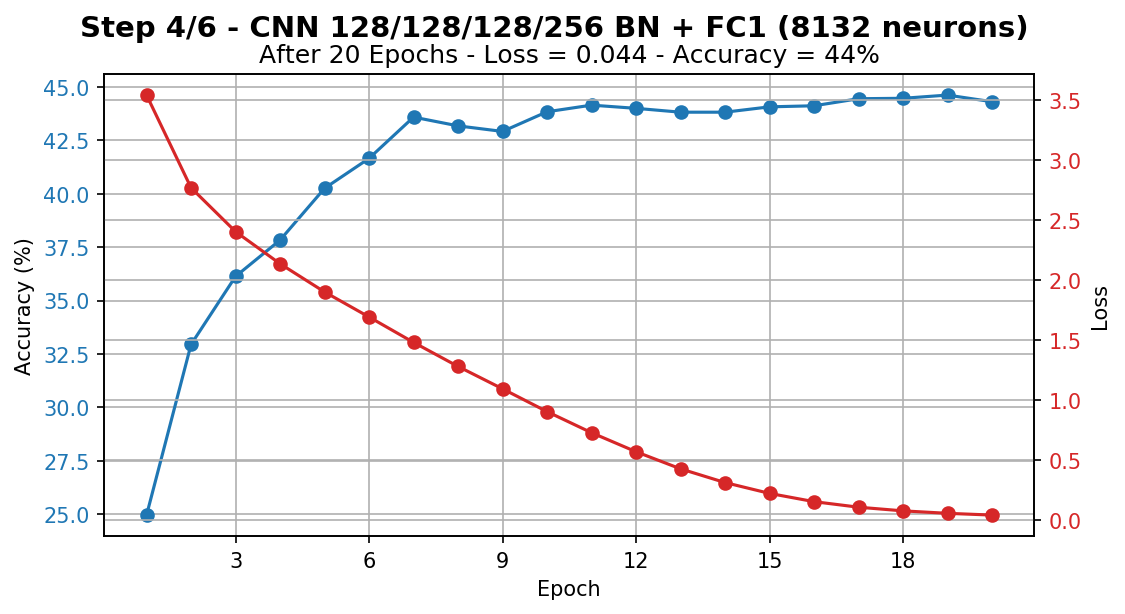
\includegraphics[width=0.62\paperwidth]{img/fig04b.png}
		\caption{CNN with Batch Normalization and FC1 wider (loss/accuracy graph)}
		\label{fig:04b}
	\end{figure}

	\begin{figure}[ht!]
		\centering
		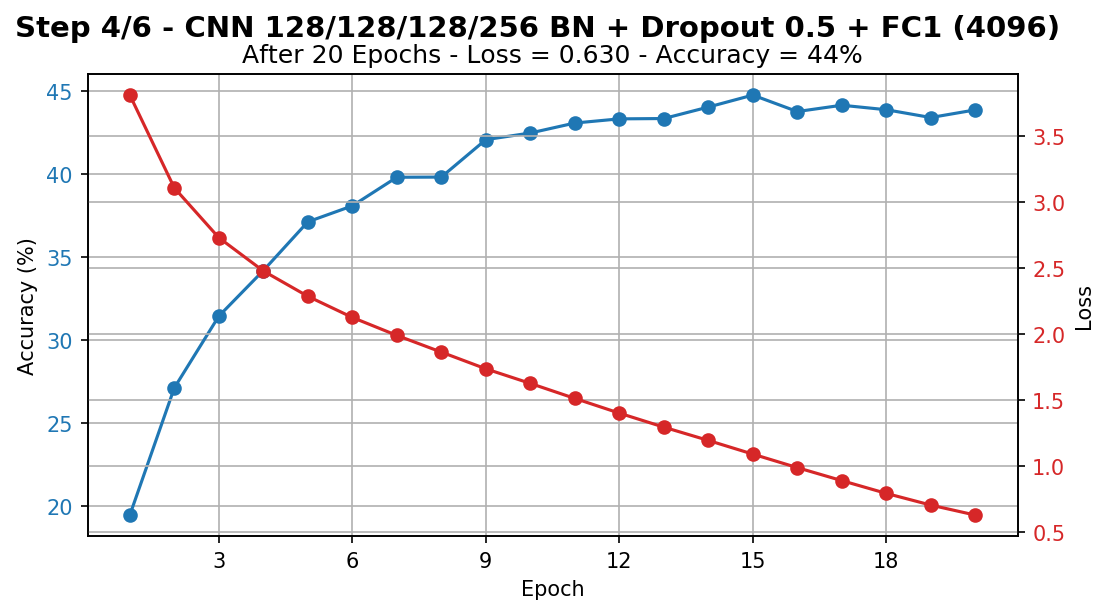
\includegraphics[width=0.62\paperwidth]{img/fig04c.png}
		\caption{CNN with Batch Normalization and Dropout $0.5$ on FC1 (loss/accuracy graph)}
		\label{fig:04c}
	\end{figure}
	\FloatBarrier
	\newpage
	The training lasted about $10$ minutes for the first CNN ($\boldsymbol{43\%}$ accuracy, $\boldsymbol{0.140}$ loss)  , $12$ minutes for the second one ($\boldsymbol{44\%}$ accuracy, $\boldsymbol{0.044}$ loss) and $10$ minutes for the last one ($\boldsymbol{44\%}$ accuracy, $\boldsymbol{0.630}$ loss): the results can be seen in \vref{fig:04a,fig:04b,fig:04c}.
	These data are better than the previous CNN ones in terms of accuracy ($10\%$ higher), while the loss is almost as low as before. 
	These results are better, because we used regularization and improving techniques.
	
	\textbf{Batch Normalization} is useful to normalize the data after each convolutional layer. We have to do this because, after each convolutional layer, the data is not normalized anymore and this slows down the process bringing convergence and the \textbf{Vanishing Gradient} problems. The mean and the variance is not know, but can be calculated on each batch of data at training time. Thanks to this, the network  learns means and variances and it uses them to approximate true mean and variance of the dataset.
	
	\textbf{Dropout} is useful to prevent overfitting and co-adaptation. It consists in randomly dropping-out some neurons at training time with a specified rate. This is done usually on FC layers, which are the ones where co-adaptation is more frequent. 
	
	\section{Data Augmentation techniques}
	
	In the fifth part of this homework I trained a CNN architecture using different types of data augmentation the network with $128$/$128$/$128$/$256$ filters. The parameters were: \textbf{256 batch size}, \textbf{20 epochs}, \textbf{32x32 resolution} for random horizontal flipping, \textbf{40x40 resolution} for random crop, \textbf{$\boldsymbol{0.0001}$ Adam Solver learning rate}. The training transformation composition on these networks can be found in \vref{lst:cnn5a,lst:cnn5b}.
	
	\lstinputlisting[aboveskip=1pt, linerange={162-168}, firstnumber=162,label={lst:cnn5a},caption={Random Horizontal Flipping in training data (\texttt{CNN5a.py})}, belowskip=0pt]{../source_code/CNN5a.py}
	\lstinputlisting[aboveskip=1pt,linerange={162-168}, firstnumber=162,label={lst:cnn5b},caption={Random Crop on training data (\texttt{CNN5b.py})}]{../source_code/CNN5b.py}
	
	The training lasted about $10$ minutes for \textbf{Random Horizontal Flipping} ($\boldsymbol{36\%}$ accuracy, $\boldsymbol{0.977}$ loss)  and $10$ minutes for \textbf{Random Crop} ($\boldsymbol{33\%}$ accuracy, $\boldsymbol{2.107}$ loss) and the results are illustrated in \vref{fig:05a,fig:05b}.
	These are better than the CNN of \cref{sect2} in terms of accuracy, because with data augmentation the CNN applies random variations on the original dataset, which can be seen as noise useful to prevent overfitting.
	
	\textbf{Random Horizontal Flipping} is a simple modification that increases accuracy almost without affecting training complexity, indeed the final loss value in our experiment was low. 
	Instead, \textbf{Random Crop} is still a simple modification, but it affects training complexity, see the high final loss value, in order to obtain a better accuracy in test time.  
	
	Taking all the arguments into account, \textbf{Random Horizontal Flipping} is the type of data augmentation which leads to better results in this case.
	
	\begin{figure}[ht!]
		\centering
		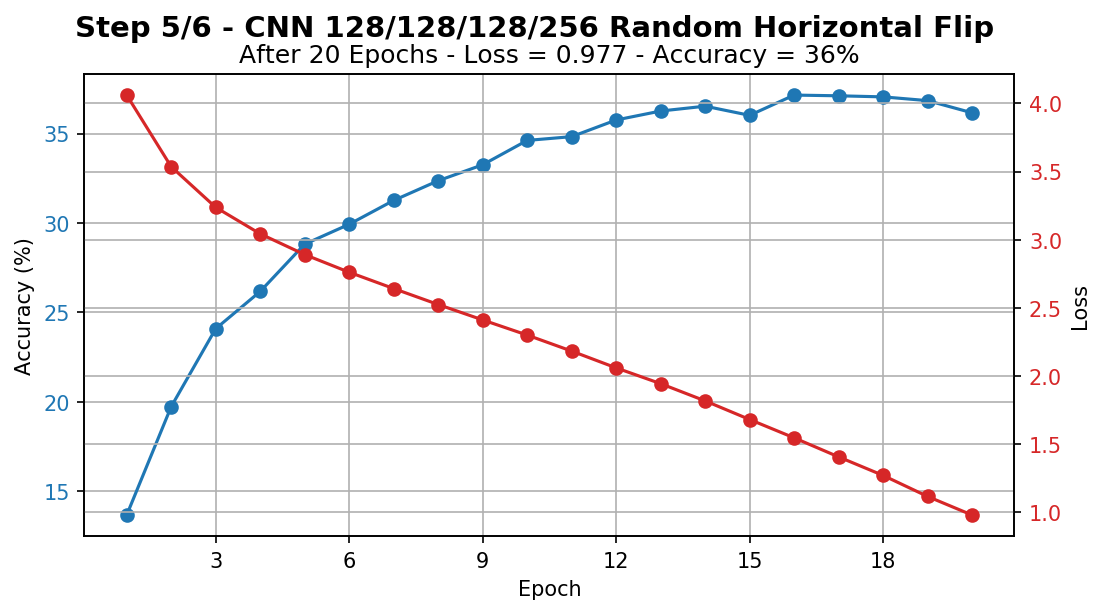
\includegraphics[width=0.65\paperwidth]{img/fig05a.png}
		\caption{CNN with Random Horizontal Flipping (loss/accuracy graph)}
		\label{fig:05a}
	\end{figure}
	\begin{figure}[ht!]
		\centering
		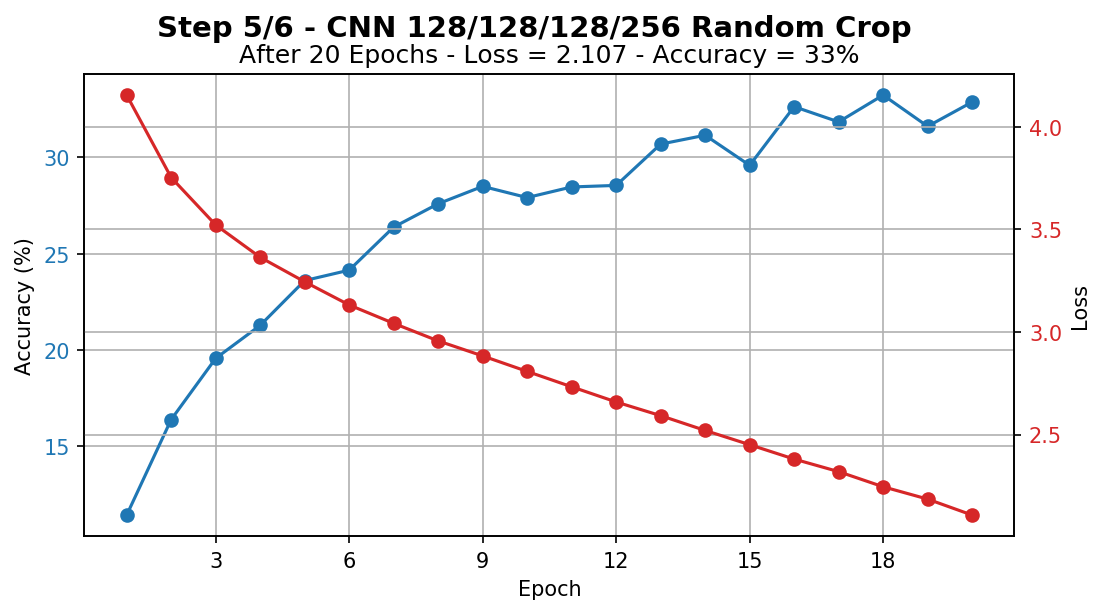
\includegraphics[width=0.65\paperwidth]{img/fig05b.png}
		\caption{CNN with Random Crop (loss/accuracy graph)}
		\label{fig:05b}
	\end{figure}
	\FloatBarrier	
	
	\section{ResNet18} \label{final}
	
	In the last part of this homework, I performed finetuning using Random Horizontal Flipping on \textbf{ResNet18} pretrained on \textit{ImageNet}. The parameters were: \textbf{128 batch size}, \textbf{10 epochs}, \textbf{224x224 resolution} and \textbf{$\boldsymbol{0.0001}$ Adam Solver learning rate}.
	
%	\lstinputlisting[aboveskip=1pt, linerange={29-35}, firstnumber=29,label={lst:cnn5a},caption={Random Horizontal Flipping in training data}, belowskip=0pt]{../source_code/CNN5a.py}
%	\lstinputlisting[aboveskip=1pt,linerange={34-40}, firstnumber=34,label={lst:cnn5b},caption={Random Crop on training data}]{../source_code/CNN5b.py}
	
	The training lasted about $1$ hour and $40$ minutes with an accuracy of $\boldsymbol{80\%}$ and a loss of $\boldsymbol{0.049}$ as we can see in \vref{fig:06}.
	As it is expected, the accuracy is very high and the loss is near to zero, so the ResNet18 produced very valuable results.
	
	It is easy to notice that the curve of loss goes to zero faster than other ones in all graphs of this report.
	This is a characteristics of ResNet18, which probably derives by its model (see \vref{fig:resnet}). A Residual Network is able to keep the gradient clean and avoid \textbf{Vanishing Gradient Problem} and, thanks to this, it can leads to better results.
	
	
	\begin{figure}[ht!]
		\centering
		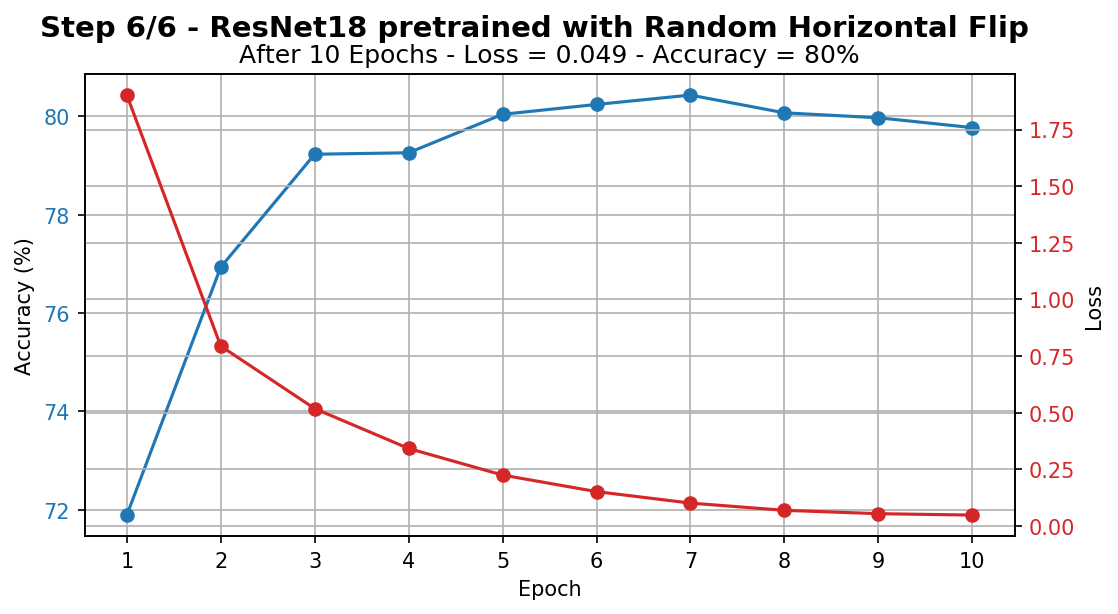
\includegraphics[width=0.62\paperwidth]{img/fig06.png}
		\caption{ResNet18 pretrained with Random Horizontal Flipping (loss/accuracy graph)}
		\label{fig:06}
	\end{figure}

\begin{figure}[ht!]
	\centering
	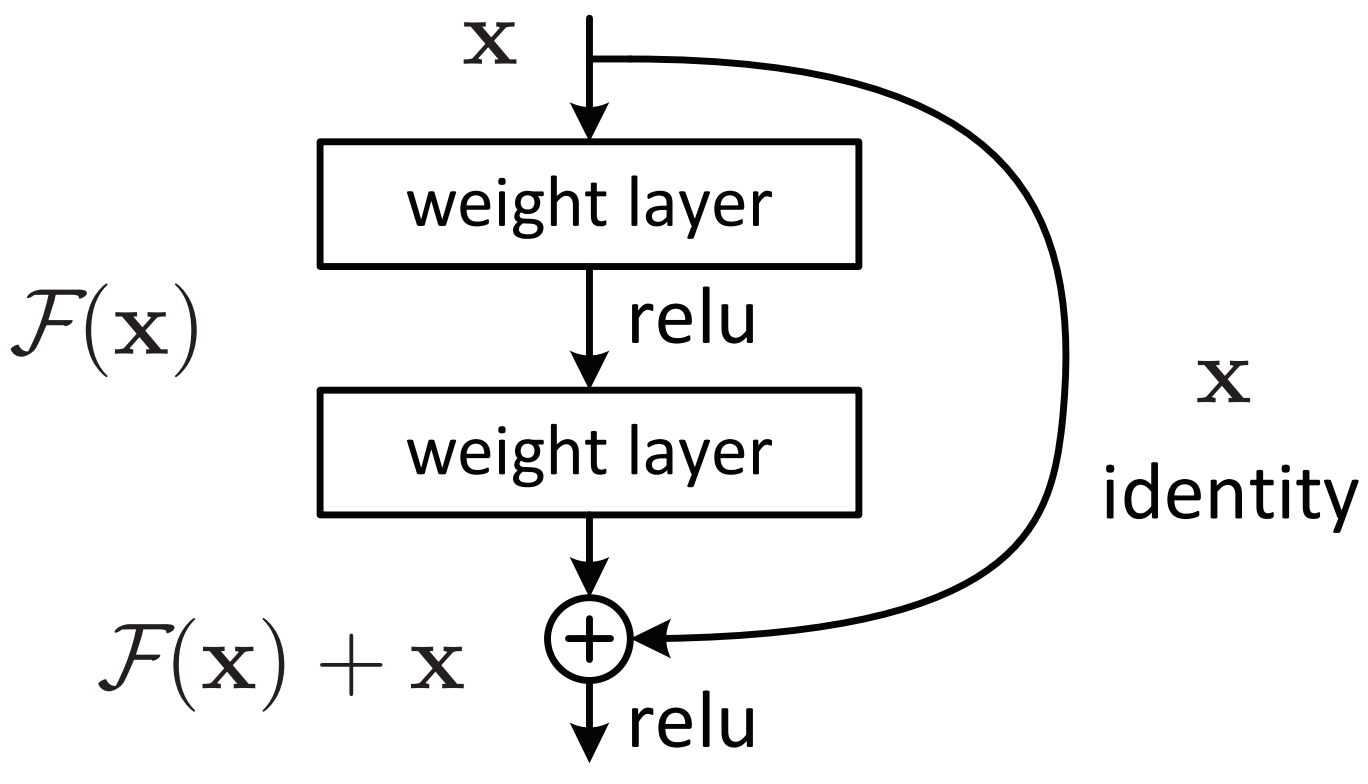
\includegraphics[width=0.3\paperwidth]{img/res.png}
	\caption{Residual Network: connection skipping}
	\label{fig:resnet}
\end{figure}

	\FloatBarrier
	
	\section{Plotting Kernel and Output}
	
	I modified the functions provided in the original code (see \texttt{plotting2.py} and \texttt{plotting6.py}) in order to plot \textbf{kernels} and \textbf{output} of the \textbf{first convolutional layer} of the CNN of \cref{sect2} and the ResNet18 of \cref{final}. The results are shown in \vref{fig:07,fig:07a,fig:07b}.
	
	It is easy to notice in \cref{fig:07a} that the kernels of the first CNN don't describe a regular and particular shape because they have not been trained yet. On the other hand, the kernels of ResNet18 show particular patterns and shapes because they have already been trained.
	
	For this reason, it is possible to distinguish the original images in the outputs of ResNet18, while it is more difficult with the results of the Simple CNN. 
	
	Analyzing \cref{fig:07bb}, it is noticeable that every kernel in the ResNet (but in general in all CNN) highlights different aspects of the same image in order to extract features, even those invisible to the human eye. 
	
	\begin{figure}[h!]
		\centering

		\begin{subfigure}[h]{0.5\textwidth}
			\centering
			\includegraphics[width=1.2in]{img/fig07a.png}
			\caption{32x32 bit resolution}
		\end{subfigure}%
		~ 
		\begin{subfigure}[h]{0.5\textwidth}
			\centering
			\includegraphics[width=1.2in]{img/fig07b.png}
			\caption{224x224 bit resolution}
		\end{subfigure}
		
		\caption{Image of the CIFAR-100 used}
		\label{fig:07}
	\end{figure}

\clearpage

	
	\begin{figure}[h!]
		\centering
		\begin{subfigure}[b]{1\textwidth}
			\centering
			\includegraphics[width=1\linewidth]{img/fig07a1.png}
			\caption{Simple CNN}
		\end{subfigure}
	
		\begin{subfigure}[b]{1\textwidth}
			\centering
			\includegraphics[width=1\linewidth]{img/fig07b1.png}
			\caption{ResNet18}
		\end{subfigure}
		\caption{Kernels of First Convolutional Layer}
		\label{fig:07a}
	\end{figure}
\clearpage

	\begin{figure}[h!]
		\centering
		\begin{subfigure}[b]{1\textwidth}
			\centering
			\includegraphics[width=1\linewidth]{img/fig07a2.png}
			\caption{Simple CNN}
		\end{subfigure}
		
		\begin{subfigure}[b]{1\textwidth}
			\centering
			\includegraphics[width=1\linewidth]{img/fig07b2.png}
			\caption{ResNet18}
			\label{fig:07bb}
		\end{subfigure}
		\caption{Outputs of First Convolutional Layer}				\label{fig:07b}
	\end{figure}
	

	
	\clearpage
	\section{Code Execution}
	\subsection{Requirements}
	\begin{itemize}
		\item Python 3
		\item All dependencies in \texttt{requirements.txt}.
		
		\texttt{\$ pip install -r requirements.txt} to install them
	\end{itemize}
	\subsection{Usage}
	\begin{itemize}
		\item \texttt{\$ python main.py <python\_script\_cnn>}
		
		Execute the script of the specified \texttt{<python\_script\_cnn>} path among these: \\
		STEP 1: NN1.py\\
		STEP 2: CNN2.py\\
		STEP 3: CNN3a.py or CNN3b.py or CNN3c.py\\
		STEP 4: CNN4a.py or CNN4b.py or CNN4c.py\\
		STEP 5: CNN5a.py or CNN5b.py\\
		STEP 6: CNN6.py\\
		STEP 7: plotting2.py or plotting6.py\\
		
	\end{itemize}
	
	\section*{Attachments}
	%Make sure to change these
	\begin{itemize}
		\item \texttt{source\_code} folder:
		\begin{itemize}
			\item \texttt{main.py}
			\item \texttt{requirements.txt}
			\item \texttt{NN1.py} - First Step Source Code
			\item \texttt{CNN2.py} - Second Source Code
			\item \texttt{CNN3a.py}, \texttt{CNN3b.py}, \texttt{CNN3c.py} - Third Step Source Codes
			\item \texttt{CNN4a.py}, \texttt{CNN4b.py}, \texttt{CNN4c.py} - Fourth Step Source Codes
			\item \texttt{CNN5a.py}, \texttt{CNN5b.py} - Fifth Step Source Codes
			\item \texttt{CNN6.py} - Sixth Step Source Codes
			\item \texttt{plotting2.py}, \texttt{plotting6.py} - Optional step of the homework
		\end{itemize}
	\end{itemize}
	%\fi %comment me out

	
\end{document}
